\iffalse
\title{Assignment12}
\author{ee24btech11064}
\chapter{2022}
\section{xe}
\fi

%\begin{enumerate}
    \item For a binary system at constant pressure, there are two types of invariant reactions:
    \[
    \text{(i) } \alpha \leftrightarrow \beta + \gamma \quad \text{(ii) } \alpha + \beta \leftrightarrow \gamma
    \]
    Analogously, how many different types of invariant reactions may exist under variable temperature and pressure, for a binary system?
    \begin{multicols}{2}
    \begin{enumerate}
            \item 1
            \item 2
             \item 3
            \item 4
    \end{enumerate}
    \end{multicols}
    \bigskip
\item For a glass marginally below its glass transition temperature, which one of the following statements is true?
\begin{enumerate}
        \item Glass has higher enthalpy than both the corresponding crystalline and liquid phases
        \item Glass has lower enthalpy than both the corresponding crystalline and liquid phases
        \item Glass has higher entropy than the corresponding crystalline phase and lower entropy than the corresponding liquid phase
        \item Glass has lower entropy than the corresponding crystalline phase and higher entropy than the corresponding liquid phase
\end{enumerate}
\bigskip
\item Which one of the following samples of high-purity aluminium (Al) single crystal will plastically yield at the lowest applied load under ambient conditions? The loading axis is along the direction shown in the schematic.
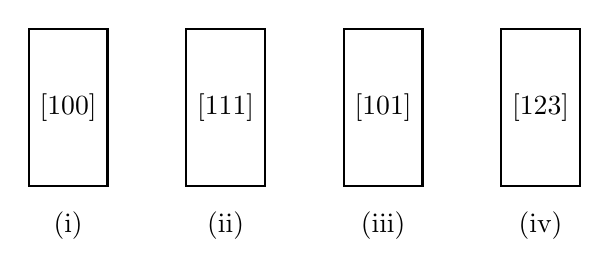
\begin{tikzpicture}

% Manually define each rectangle and its label to avoid issues with undefined control sequences
% First rectangle
\draw[thick] (0,0) rectangle ++(1,2);
\node at (0.5,1) {[100]};
\node at (0.5,-0.5) {(i)};

% Second rectangle
\draw[thick] (2,0) rectangle ++(1,2);
\node at (2.5,1) {[111]};
\node at (2.5,-0.5) {(ii)};

% Third rectangle
\draw[thick] (4,0) rectangle ++(1,2);
\node at (4.5,1) {[101]};
\node at (4.5,-0.5) {(iii)};

% Fourth rectangle
\draw[thick] (6,0) rectangle ++(1,2);
\node at (6.5,1) {[123]};
\node at (6.5,-0.5) {(iv)};

\end{tikzpicture}
\begin{multicols}{2}
    \begin{enumerate}
        \item (i)
        \item  (ii)
        \item (iii)
        \item (iv)
    \end{enumerate}
\end{multicols}
\bigskip
\item Refer to the schematic shown. Two dog-bone samples, labeled 1 and 2, of a Cu-alloy are tested under tension at room temperature to points E and P, respectively. Subsequently, they are unloaded completely and metallographically polished. Brinell hardness testing was performed in the gauge section of the samples. Which one of the following can be inferred about the measured Brinell hardness number (BHN)?
\begin{figure}[H]
\centering
\resizebox{0.5\textwidth}{!}{%
\begin{circuitikz}
\tikzstyle{every node}=[font=\Large]
\draw [->, >=Stealth] (4.75,7.5) -- (4.75,10.5);
\draw [->, >=Stealth] (4.75,7.5) -- (7.75,7.5);
\draw [dashed] (5,7.5) -- (6.5,10);
\draw [short] (4.75,7.5) .. controls (6.5,11) and (6.75,9.5) .. (7.75,10);
\node [font=\LARGE] at (4.25,9.75) {$\sigma$};
\node [font=\normalsize] at (5.25,9.25) {E};
\node [font=\normalsize] at (7.25,9.5) {P};
\node [font=\Large] at (7,7.25) {$\epsilon$};
\end{circuitikz}
}%

\end{figure}
\begin{enumerate}
    \begin{multicols}{2}
        \item BHN of 1 $>$ BHN of 2
        \item BHN of 1 = BHN of 2
        \item BHN of 1 $<$ BHN of 2
        \item Cannot be concluded with provided information
    \end{multicols}
\end{enumerate}
\bigskip
\item During the ageing of a homogenized Al-Cu alloy (1 to 4 wt.\% Cu) below the GP zone solvus, hardness of the alloy:
\begin{enumerate}
        \item increases monotonically
        \item decreases monotonically
        \item first increases then  decreases
        \item first decreases then incrases 
\end{enumerate}
\bigskip
\item A student aims to deposit a thin metallic film on a SiO$_2$ substrate, with an adhesion layer between the metal film and substrate, in a contiguous planar fashion. Island-type growth must be avoided. Which one of the following steps is in the right direction?
\begin{enumerate}

        \item Choose a metallic adhesion layer with very low interfacial energy with the deposited thin film
        \item Choose a metallic adhesion layer with very low interfacial energy with SiO$_2$, irrespective of its interaction with the metal film
        \item Increase the substrate temperature and decrease the deposition rate
        \item Use intermittent stages of deposition followed by annealing

\end{enumerate}
\bigskip
\item For a diffusional transformation (i.e., growth of $\beta$ precipitates in an $\alpha$ matrix), which of the following is/are true with increasing degree of undercooling? 
\begin{enumerate}
    \item Rate of transformation first increases and then decreases
    \item Rate of transformation first decreases and then increases
    \item Thermodynamic driving force increases monotonically
    \item Mobility of atoms in $\alpha$ matrix remains unchanged

\end{enumerate}
\bigskip
\item A two-phase ($\alpha + \beta$) mixture of an A-B binary system has the following properties:
\begin{enumerate}

        \item Phase $\alpha$ has equal weight percentages of A and B.
        \item Phase $\beta$ has twice the mole fraction of A compared to B.
        \item The two-phase mixture has equal amounts of $\alpha$ and $\beta$.
        \item Atomic mass of A is twice that of B.
    
\end{enumerate}
The mole fraction of A in the resultant two-phase mixture is \underline{\hspace{1cm}}
\bigskip
\item It is known that component A diffuses into a solid to a depth of $10 \, \mu$m in 1 hour at 300 K. The time taken for A to diffuse to the same depth at 600 K is \underline{\hspace{1cm}} seconds. (Round off to one decimal)
Diffusivity of A in the solid is given by 
\begin{align*}
    D_{A}=D_{A}^\circ exp(\frac{-E_{a}}{k_b T})
\end{align*}
$D_{A}$: Diffusivity Coefficient \\
$E_a$: Activation energy = 0.3ev \\
$k_b$: Boltzmann's Constant = 8.62 $\times 10^{-5} eV/K$\\
$T$ : Absolute Temperature 
\bigskip
\item A spherical $\beta$ particle nucleates from the $\alpha$ matrix on a non-deformable substrate $\delta$. forming a contact angle of $\theta$ as shown in the schematic\\
	The value of $\frac{\Delta \text{G}_{\text{het}}}{\Delta \text{G}_{\text{hom}}}$ is \underline{\hspace{1cm}}. (Round off to three decimal places)
\begin{figure}[H]
\centering
\resizebox{0.3\textwidth}{!}{%
\begin{circuitikz}
\tikzstyle{every node}=[font=\normalsize]
\draw [short] (4.25,10.75) -- (8.5,10.75);
\draw [short] (4.25,10.75) -- (4.25,6);
\draw [short] (4.25,6) -- (8.5,6);
\draw [short] (8.5,6) -- (8.5,10.75);
\draw [short] (4.25,8) -- (8.5,8);
\draw [dashed] (5.25,8) -- (6,9.5);
\draw [short] (5.25,8) .. controls (5.75,9.25) and (6.75,9) .. (7.25,8);
\draw [dashed] (5.75,8) .. controls (5.75,8.25) and (5.75,8.25) .. (5.5,8.25);
\node [font=\normalsize] at (6,8.25) {$\theta$};
\node [font=\normalsize] at (6.25,10) {$\alpha$};
\node [font=\normalsize] at (6.25,8.5) {$\beta$};
\node [font=\normalsize] at (6.25,7) {$\delta$};
\end{circuitikz}
}%

\end{figure}
$\Delta G^*_{\text{hom}}$ = Gibbs free energy change at the critical radius for homogeneous nucleation \\
$\Delta G^*_{\text{het}}$ = Gibbs free energy change at the critical radius for heterogeneous nucleation \\
$\alpha-\beta$ interfacial energy = $0.4 J/m^2$ \\
$\alpha-\delta$ interfacial energy = $0.3 J/m^2$ \\
$\beta-\delta$ interfacial energy = $0.02 J/m^2$ \\

\bigskip
\item The resistivity of a pure semi-conductor at 298 K is $300\Omega m$. Assume that the number of electrons excieted ($n_e$) across the band gap is given by the relation 
\begin{align*}
    n_{e}=N_{A} exp\frac{-E_{g}}{k_B T}
\end{align*}
$N_{A}$: Avogadro's number = $6.02\times 10^{23}mole^{-1}$\\
$k_B$: Boltzmann's constant = $8.62\times 10^{-5} eV/K$\\
T: Absolute Temperature \\
Mobility of electrons in the semiconductor = $0.14 m^2/(V s)$\\
Mobility of holes iin the semiconductor = $0.06 m^2/(V s)$\\
Absolute charge of an electron = $1.60\times10^{-19}C$\\
The band gap ($E_g$) of the semiconductor is \underline{\hspace{1cm}} eV. (Round off to two decimals)
\bigskip
\item A new glass material is developed to minimize the transmission of light through a window with a glass panel of thickness 5 mm. The refractive index of the glass material is 1.5 and the absorption coefficient can be changed from $0.3cm^{-1}$ to $1cm^{-1}$. IN the given range of absorption coefficients, the ratio of the maximum to the minimuum fraction of the light coming out of the other side of the glass panel is \underline{\hspace{1cm}}. (Round off to two decimal places)
\bigskip
\item The third peak in the X-ray diffraction pattern of a face-centered cubic cystal is at $2\theta$ value of $45^\circ$, where $2\theta$ is the nagle between the incident and the reflected rays. The wavelength of the monochromatic X-ray beam is $1.54 A^\circ$. Considering first-order reflection, the lattice parameter of the crystal is \underline{\hspace{1cm}}$A^\circ$. (Round off to two decimal places)
%\end{enumerate}
